\documentclass{article}

\usepackage[utf8]{inputenc}
\usepackage{amssymb}
\usepackage{amsmath}
\usepackage{mathabx}
\usepackage{dcolumn}
\usepackage{geometry}
\usepackage{breqn}
\usepackage{graphicx}
\usepackage{float}
\usepackage{mathrsfs}
\usepackage{array}
\usepackage{caption}
\usepackage{subcaption}
\usepackage[spanish,es-lcroman]{babel}
\usepackage{enumerate}
\usepackage{nicefrac} 
\usepackage[most]{tcolorbox}
\usepackage{tcolorbox} % For solution boxes
%\decimalpointf
\setlength\parindent{0pt}
\usepackage{enumitem}
\newcommand*{\QED}{\hfill\ensuremath{\blacksquare}}
%\usepackage{authblk}
\selectlanguage{spanish}
\geometry{letterpaper, margin=1in}
\pagestyle{headings}
\usepackage{amsthm} 
\newtheorem{theorem}{Teorema}[section]
\newtheorem{corollary}{Corolario}[theorem]
\newtheorem{lemma}[theorem]{Lema}
\theoremstyle{remark}
\newtheorem*{remark}{Considere}
\DeclareUnicodeCharacter{2212}{-}
\usepackage{epigraph}
\usepackage{booktabs}
\usepackage[backend=biber, style=apa]{biblatex}
\addbibresource{ref.bib}

%\usepackage[natbibapa]{apacite}
\usepackage{tikz}
\usepackage{hyperref}

\tcbset{colback=blue!10, 
    %colframe=green!45!black!20, 
    colframe=blue!70!black!70, 
    title=Soluci\'on,
    fonttitle=\bfseries,  
    coltitle=white,
    standard jigsaw, opacityback=50, arc=0mm, breakable} 

\newcommand{\ubar}[1]{\text{\b{$#1$}}}
 
\theoremstyle{definition}
\newtheorem{definition}{Definici\'on}[section]

\title{\textbf{Tendencia, Estacionalidad, Ciclos y Volatilidad} \\ {\Large Series de Tiempo para Pron\'osticos en Econom\'ia y Finanzas} \\ {\large Taller 2}}
\author{Nicolas Lozano Huertas\thanks{\href{mailto:n.lozanoh@uniandes.edu.co?subject= Taller 2 Series de Tiempo}{Universidad de los Andes}} \and Juan José Gutierrez \and Sof\'ia Prada \and Valentina Rond\'on}
\date{Abril, 2025}

\begin{document}

\maketitle
\vspace{-1 cm}
\section{[10 puntos] Modelos ARCH.}
{Lea el ``Nobel Lecture'' de Robert Engle para m\'as informaci\'on de los modelos ARCH.}
\begin{enumerate}[label = \emph{\alph*})]
    \item {Hagan un resumen de no m\'as de una p\'agina sobre esta lectura.}
        \begin{tcolorbox}[title=Soluci\'on 1.a]
            En su Nobel Lecture, \cite{engle2004}, busca exponer las principales car\'acteristicas de los modelos GARCH, su historia y algunas aplicaciones en mercados financieros. \\
            El autor comienza haciendo una breve introducci\'on en la cual resalta la importancia de medir el riesgo 
        \end{tcolorbox}
    \item {¿De acuerdo a la lectura, cu\'ales son las caracter\'isticas de los datos financieros y macroecon\'omicos que los modelos ARCH pueden capturar?}
        \begin{tcolorbox}[title=Soluci\'on 1.b]
            
        \end{tcolorbox}
\end{enumerate}

\section{[45 puntos] Pron\'ostico de Variables Financieras.}

{En el archivo de Excel que se llama ``TRM'' que se encuentra en la carpeta de este taller, se tienen los datos de la tasa representativa de mercado diaria del peso colombiano con respecto al d\'olar de Estados Unidos, desde el 1 de diciembre del año 1991 hasta el 25 de marzo del año 2025.}

\begin{enumerate}[label = \emph{\alph*})]
    \item {Construya una serie mensual hist\'orica con la TRM promedio mensual desde diciembre del año 1991 hasta marzo del año 2025. Grafiquen la serie hist\'orica de la TRM construida y analicen los hechos m\'as relevantes que han generado variaciones en la TRM en el presente siglo. No es necesario un an\'alisis exhaustivo, s\'olo los principales hechos asociados a cambios fuertes en la serie observada.}
        \begin{tcolorbox}[title=Soluci\'on 2.a]
            \begin{figure}[H]
                \centering
                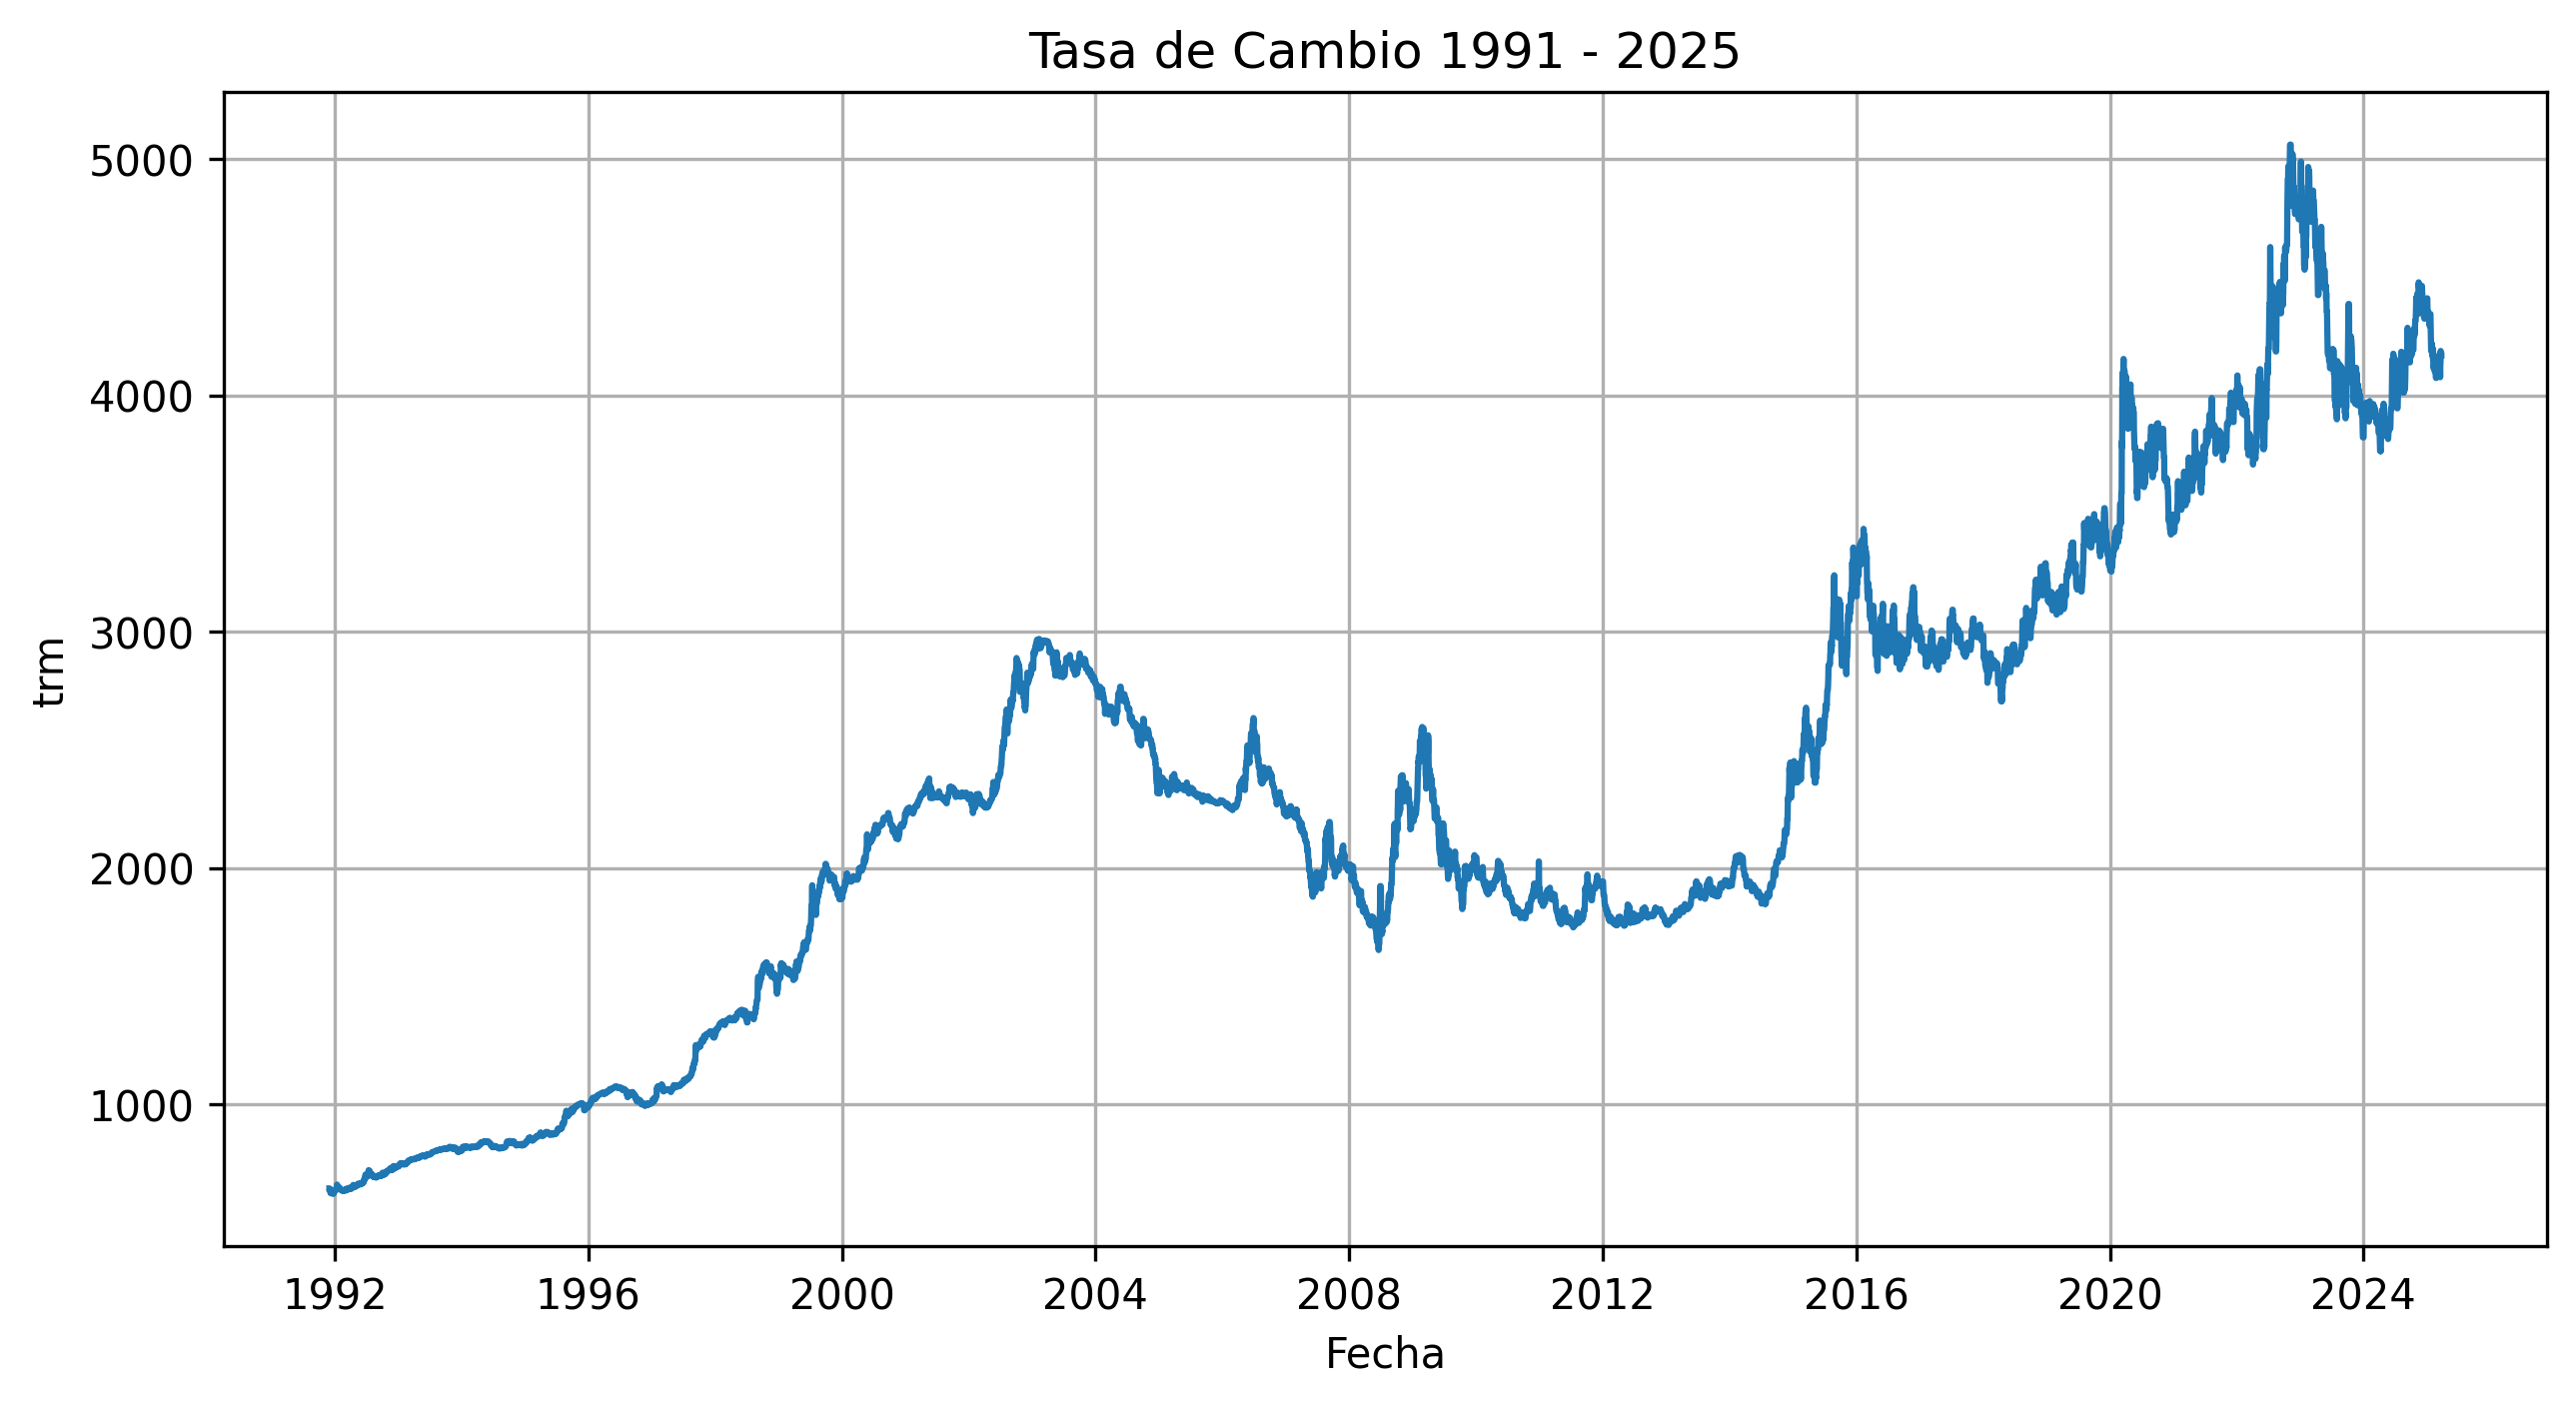
\includegraphics[width=0.9\linewidth]{output/graf_trm.png}\
                \caption{Serie TRM}
                \label{fig:serie_trm}
            \end{figure}
        \end{tcolorbox}
    \item {Estimen el retorno mensual de la TRM:}
    \begin{equation}
        r_t = (\ln(TRM_t) - \ln(TRM_{t-1})) \times 100
    \end{equation}
    {donde TRM$_t$ es la TRM promedio en el mes $t$. Calcule el valor promedio de dicha serie y rep\'ortelo. ¿En promedio los retornos de la TRM son positivos, negativos o cero?}
        \begin{tcolorbox}[title=Soluci\'on 2.b]
        
            \begin{table}[H]
\caption{Retorno Promedio}
\label{tab:retorno_promedio}
\begin{tabular}{lr}
\toprule
Estad\'istico & Valor \\
\midrule
Retorno Promedio & 0.015357 \\
\bottomrule
\end{tabular}
\end{table}

            
        \end{tcolorbox}
    \item {Estime el retorno mensual sin media y eleve dicha medida al cuadrado de la siguiente manera: }

    \begin{equation}
        r_t^2-[r_t-\bar{r}]^2
    \end{equation}

    {Donde $r_t$ es el valor de los retornos mensuales y $\bar{r}$ es el valor promedio de los retornos mensuales.} \\
    
    {Presente en dos gr\'aficas (tipo subplot) los retornos mensuales $r_t$ de la TRM y los retornos al cuadrado. Describa las gr\'aficas e interprete sus resultados a la luz de los an\'alisis realizados en clase y a partir de lo analizado en los hechos hist\'oricos descritos en el segundo apartado.}
        \begin{tcolorbox}[title=Soluci\'on 2.c]
            \begin{figure}[H]
                \centering
                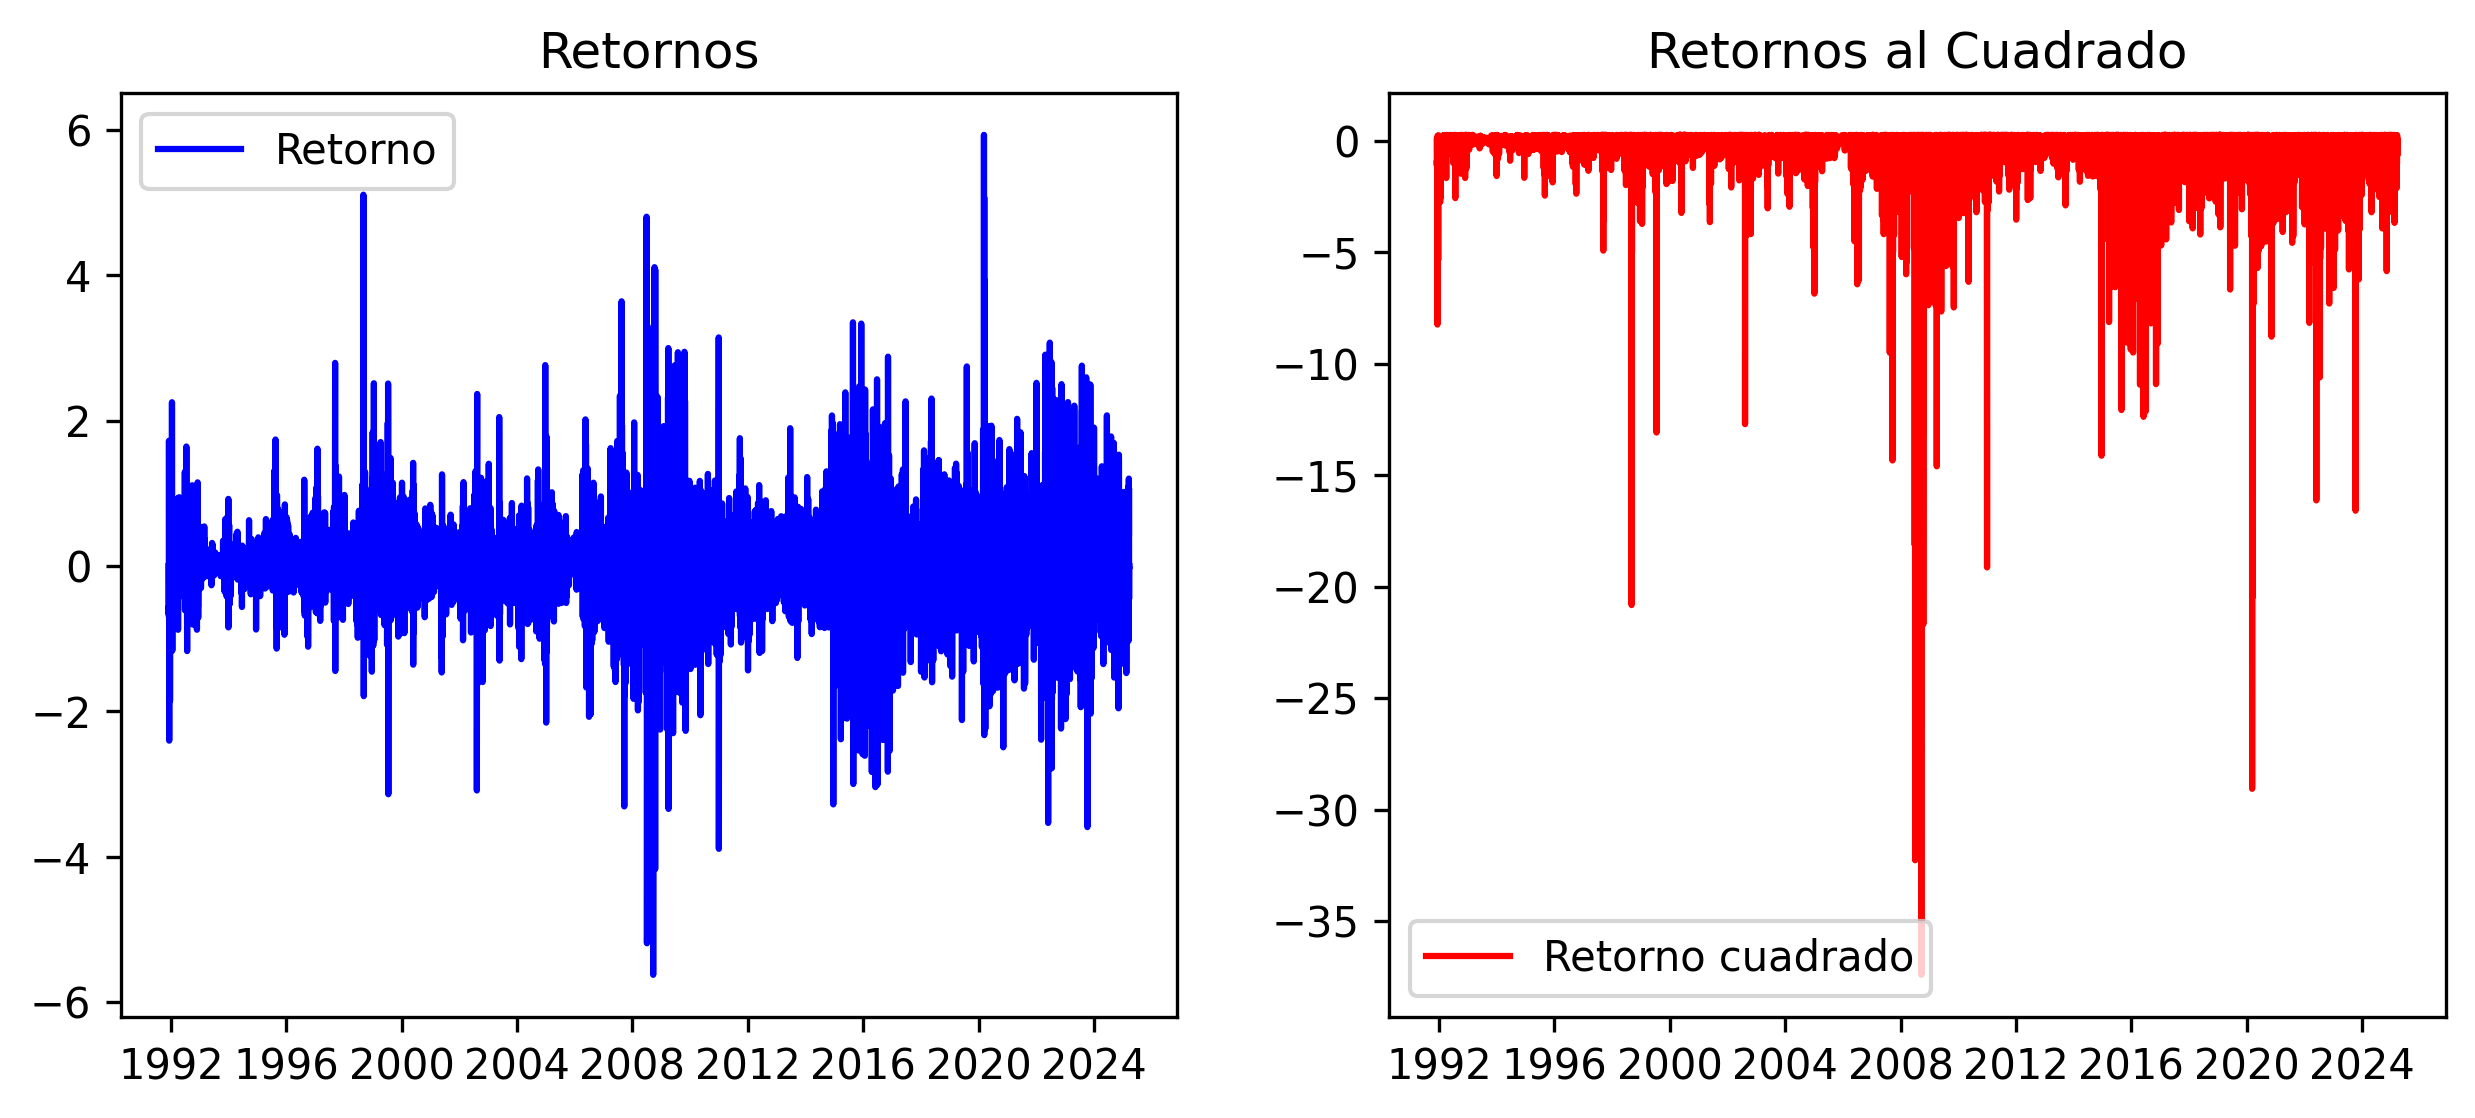
\includegraphics[width=0.9\linewidth]{output/subplot_retornos.png}
                \caption{Retornos}
                \label{fig:retorno}
            \end{figure}
        \end{tcolorbox}
\end{enumerate}

{Ahora, asuman que los datos de los retornos mensuales $r_t$ tienen una estructura de la forma:}
\begin{align*}
    \Phi(L)r_t &= \Theta(L)\varepsilon_t \\
    \Phi(L) = 1 − \phi_1L &− \phi_2L^2 − \cdots − \phi_pL^p \\
    \Theta(L) = 1 + \theta_1L &+ \theta_2L^2 + \cdots + \theta_pL^p
\end{align*}

{Por su parte el error $\varepsilon_t$ puede seguir un ruido blanco fuerte ($\varepsilon_t\sim WN(0,
\sigma^2)$) o d\'ebil ($\varepsilon_t\sim D(0,\sigma_t^2)$).}

\begin{enumerate}[label = \emph{\alph*})]\setcounter{enumi}{3}
    \item {Estime el retorno mensual de la TRM que sigue un proceso ARMA. Justifique su estimaci\'on con estad\'isticas y criterios de informaci\'on.}
        \begin{tcolorbox}[title=Soluci\'on 2.d]
            \begin{table}[H]
\label{tab:dickey_fuller}
\centering
\begin{tabular}{lr}
\toprule
 & Valor \\
\midrule
Estad\'istico DF & -12.7408 \\
p-valor & 0.0000 \\
\bottomrule
\end{tabular}
\caption{Prueba Dickey-Fuller}
\end{table}

        \end{tcolorbox}
    \item {Construya y grafique la serie de residuales. Justifique que se trata de ruido blanco. Documente pruebas de normalidad y aquellas relevantes para justificar los supuestos de su modelo.}
        \begin{tcolorbox}[title=Soluci\'on 2.e]
            
        \end{tcolorbox}
    \item {Pruebe si es necesario incluir din\'amicas de varianza condicional. De ser necesario, est\'imelas y presente sus resultados (puede probar varios modelos, pero debe presentar y continuar el desarrollo del taller con uno solo). Justifique con estad\'isticas y criterios de informaci\'on el modelo estimado.}
        \begin{tcolorbox}[title=Soluci\'on 2.f]
            
        \end{tcolorbox}
    \item {Pruebe si su modelo captura correctamente las din\'amicas de varianza. Realice y documente las pruebas necesarias.}
        \begin{tcolorbox}[title=Soluci\'on 2.g]
            
        \end{tcolorbox}
\end{enumerate}

{A usted le encanta viajar y entiende que cuando viaja al exterior su plan de vacaciones puede salir m\'as caro o m\'as barato dependiendo la TRM (en este caso retornos positivos jugar\'ian en su contra). Usted tiene $\$20.000.000$ ahorrados que est\'a dispuesto a gastarse en un fant\'astico viaje a la ciudad maravilla, pero no sabe si adquirir todo lo relacionado con el viaje en este momento o esperar hasta el primer d\'ia de mayo. Afortunadamente, usted est\'a tomando el curso de pron\'osticos y acaba de estimar un modelo que le sirve para pronosticar los retornos mensuales de la TRM y su volatilidad, lo que le ayudar\'a a tomar una decisi\'on.}

\begin{enumerate}[label = \emph{\alph*})]\setcounter{enumi}{7}
    \item {Realice el pron\'ostico punto para abril del año 2025 tanto de los retornos como de la varianza. Reporte el pron\'ostico para los dos casos e interprete los dos resultados (no se pide realizar el pronostic\'o a mano, puede usar los comandos necesarios para realizar el pron\'ostico 1 paso adelante).}
        \begin{tcolorbox}[title=Soluci\'on 2.h]
            
        \end{tcolorbox}
    \item {Con el comando apropiado simule mil pron\'osticos del retorno mensual de la TRM para el mes de abril del año 2025. Haga una gr\'afica con su estimaci\'on puntual y con la funci\'on de densidad generada a partir de simulaciones de su modelo autoregresivo de media m\'ovil, indique en la gr\'afica el intervalo del 95\% de confianza: ¿Seg\'un su pron\'ostico, para el mes de abril del año 2025, ser\'ia mejor comprar todo lo relacionado con su viaje hoy o esperar el mes de abril? ¿Con los retornos esperados pronosticados usted espera una apreciaci\'on o una depreciaci\'on del peso frente al d\'olar?}
        \begin{tcolorbox}[title=Soluci\'on 2.i]
            
        \end{tcolorbox}
    \item {Ahora, todos los valores pronosticados de los retornos de la TRM para el mes de abril del año 2025 calculados en el item anterior, multipl\'iquelos por $\$20.000.000$, con esto obtendr\'a un vector de lo que ganar\'ia (si hay apreciaci\'on) y lo que perder\'ia (si hay depreciaci\'on) si decide esperar un mes y comprar todo lo relacionado con su viaje. Haga una gr\'afica con su estimaci\'on puntual y con la funci\'on de densidad generada a partir de las estimaciones, indique en la gr\'afica el intervalo del 95\% de confianza: ¿Seg\'un su pron\'ostico, usted esperar\'ia o mejor comprar\'ia todo lo relacionado con su viaje en este momento? ¿Teniendo en cuenta todo lo anterior invertir\'ia su dinero en activos asociados a la TRM peso d\'olar? ¿usar\'ia estos modelos para tomar este tipo de decisiones o mejor se guiar\'ia en su experiencia previa como turista?}
        \begin{tcolorbox}[title=Soluci\'on 2.j]
            
        \end{tcolorbox}
\end{enumerate}

\section{[45 puntos] Juntando Componentes.}

{Ahora debe pronosticar las remesas de los trabajadores trimestrales en pesos colombianos. Para esto, asuma que las series pueden seguir el modelo general visto en clase que incluye tendencia, estacionalidad, ciclos y din\'amicas de varianza.}

\begin{align*}
    y_t = T_t(\theta) +& \sum_{i=1}^{s} \gamma_i D_{it} + \varepsilon_t \\
    \Phi(L) \varepsilon_t =& \Theta(L) v_t \\
    \Phi(L) = 1 - \phi_1 L -& \phi_2 L^2 - \dots - \phi_p L^p \\
    \Theta(L) = 1 + \theta_1 L +& \theta_2 L^2 + \dots + \theta_p L^p
\end{align*}

{Por su parte el error $v_t$ puede seguir un ruido blanco fuerte ($v_t\sim WN(0,
\sigma^2)$) o d\'ebil ($v_t\sim D(0,\sigma_t^2)$).} \\

{En el archivo de Excel denominado remesas que acompaña este taller se encuentra una serie trimestral de las remesas en millones de d\'olares desde el primer trimestre del año 2000 hasta el cuarto trimestre de 2025.}

\begin{enumerate}[label=\emph{\alph*})]
    \item {Convierta los valores en d\'olares a valores en pesos, multiplic\'andolo por la TRM trimestral promedio de cada trimestre. Grafique los datos trimestrales obtenidos en pesos. Describa la din\'amica de las series trimestrales de las remesas que ustedes construyeron que est\'an denominadas en pesos colombianos. ¿Observan un cambio de tendencia de la serie a trav\'es del tiempo? Escriban expl\'icitamente si los datos trimestrales est\'an en millones de pesos, en miles de millones de pesos o en billones de pesos.}
        \begin{tcolorbox}[title=Soluci\'on 3.a]
            
        \end{tcolorbox}
    \item {Discuta, a la luz de la teor\'ia econ\'omica y financiera, cu\'ales de los componentes son relevantes para incluir en su modelo.}
        \begin{tcolorbox}[title=Soluci\'on 3.b]
            
        \end{tcolorbox}
    \item {Pruebe si es necesario incluir los componentes de tendencia y estacionalidad. De ser necesario, est\'imelos y presente sus resultados (puede probar varios modelos, pero debe continuar el desarrollo del taller con uno solo). Justifique con estad\'isticas y criterios de informaci\'on el modelo estimado.}
        \begin{tcolorbox}[title=Soluci\'on 3.c]
            
        \end{tcolorbox}
    \item {Construya y grafique la serie desestacionalizada y sin tendencia.}
        \begin{tcolorbox}[title=Soluci\'on 3.d]
            
        \end{tcolorbox}
    \item {Pruebe si es necesario incluir un componente c\'iclico. De ser necesario, estime conjuntamente el modelo con todos los componentes necesarios y presente sus resultados (puede probar varios modelos, pero debe continuar el desarrollo del taller con uno solo). Justifique con estad\'isticas y criterios de informaci\'on el modelo estimado.}
        \begin{tcolorbox}[title=Soluci\'on 3.e]
            
        \end{tcolorbox}
    \item {Construya y grafique los residuales. Justifique que se trata de ruido blanco. De ser necesario, documente las pruebas que le dan validez a sus resultados.}
        \begin{tcolorbox}[title=Soluci\'on 3.f]
            
        \end{tcolorbox}
    \item {Pruebe si es necesario incluir din\'amicas de varianza condicional. De ser necesario, est\'imelas y presente sus resultados (puede probar varios modelos, pero debe continuar el desarrollo del taller con uno solo). Justifique con estad\'isticas y criterios de informaci\'on el modelo estimado.}
        \begin{tcolorbox}[title=Soluci\'on 3.g]
            
        \end{tcolorbox}
    \item {Pruebe si su modelo captura correctamente las din\'amicas de varianza. Realice y documente las pruebas necesarias.}
        \begin{tcolorbox}[title=Soluci\'on 3.h]
            
        \end{tcolorbox}
    \item {Realice el pron\'ostico puntual trimestral y simule 1.000 pron\'osticos para todo el año 2025 (i.e. pronostique los valores trimestrales de las remesas desde el primer trimestre hasta el cuarto trimestre de 2025). Sumando dichos pron\'osticos puede obtener el valor total de las remesas esperados en el año 2025. Con este valor reporte:}
    \begin{enumerate}[label=(\emph{\roman*})]
        \item {Pron\'ostico punto del total de remesas para el año 2025.}
            \begin{tcolorbox}[title=Soluci\'on 3.i.i]
            
            \end{tcolorbox}
        \item {Pron\'ostico de intervalo al 95\% de confianza del total de remesas para el año 2025.}
            \begin{tcolorbox}[title=Soluci\'on 3.i.ii]
            
            \end{tcolorbox}
        \item {Pron\'ostico de densidad del total de remesas para el año 2025. Presente sus resultados en un gr\'afico donde pueda leerse el valor de los pron\'osticos (\emph{i}) y (\emph{ii}).}
            \begin{tcolorbox}[title=Soluci\'on 3.i.iii]
            
            \end{tcolorbox}
    \end{enumerate}
\end{enumerate}

\nocite{*}

\printbibliography

\end{document}

